\section{Introduction}
\label{sec:intro}

Crowdsourcing provides an inexpensive and efficient method to annotate data for various machine learning tasks
by employing a massive workforce from global Internet users.
Popular online crowdsourcing platform include
Amazon Mechanical Turk\footnote{\url{https://www.mturk.com/}} and CrowdFlower\footnote{\url{http://www.crowdflower.com/}}.
However, in contrast to expert annotated data,
crowdsourced annotation usually suffers from relatively higher level of errors.
%which limits the adoption of crowdsourcing as a regular method of annotated data collection.


Typically in practice, multiple questions or data items are grouped into batches
to be sent to workers on crowdsourcing platforms.
Firstly, sending batches of data items can save cost,
as the necessary instructions or background for completing the tasks can be provided only once,
which can prevent the overhead when the workers have to read elaborate instructions or background before labeling each data item.
Consider an example where the worker has to judge whether a comment is relevant to a certain document,
where making a judgment on each comment requires reading through the entire document.
Moreover, from the workers' point of view,
it is also more attractive to label batches of data items
as they can save time on switching between different tasks.
And also, once they start on a batch,
they no longer have to ``fight'' for other high paying or attractive tasks.
%


\begin{figure*}[!t]
  \centering
  %\begin{subfigure}[b]{0.62\columnwidth}
  \subfigure[Data items judged independently]{
    \label{subfig:example_ind}
   % \centering
    \begin{tabular}{@{}cc@{}}
    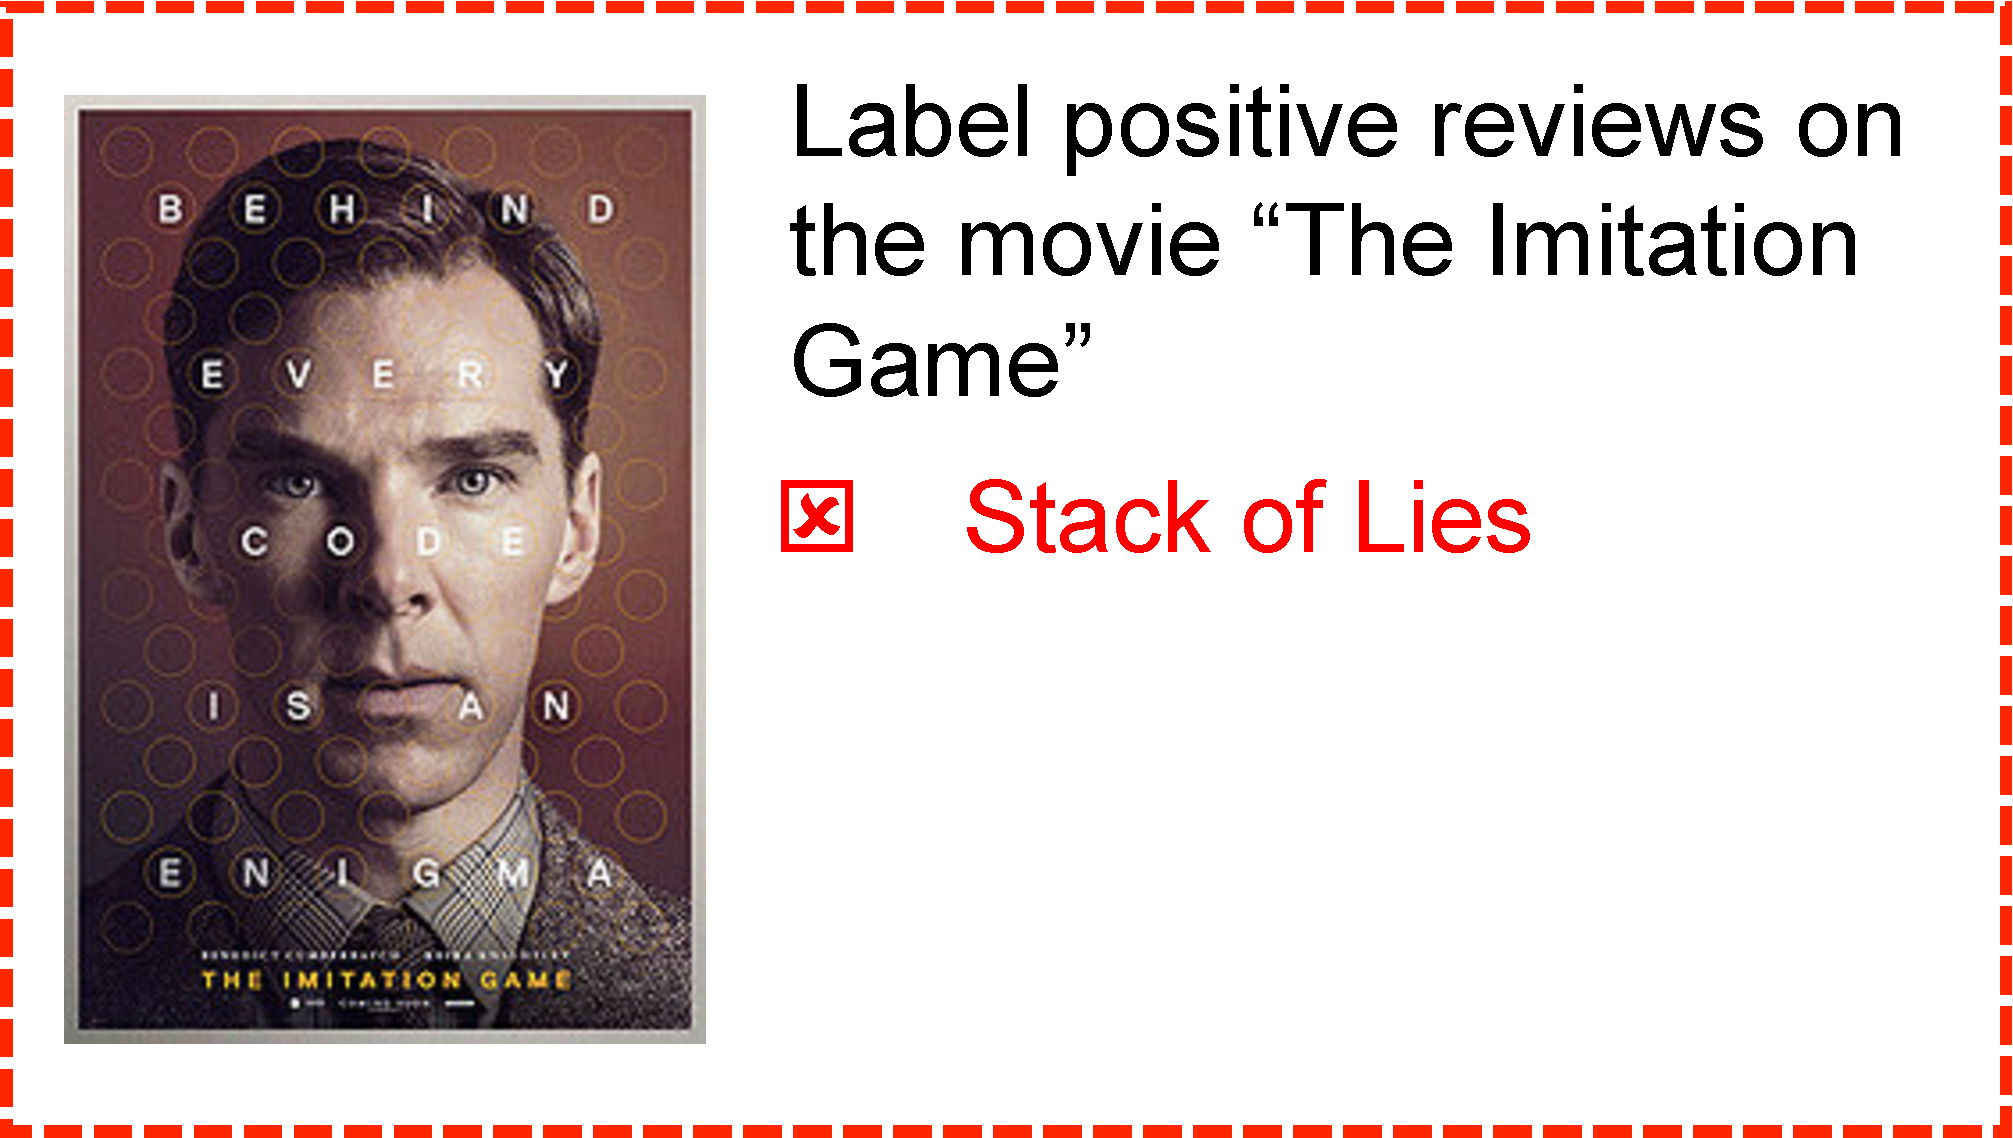
\includegraphics[width=0.30\textwidth]{figures/example_movie_ind1} &
    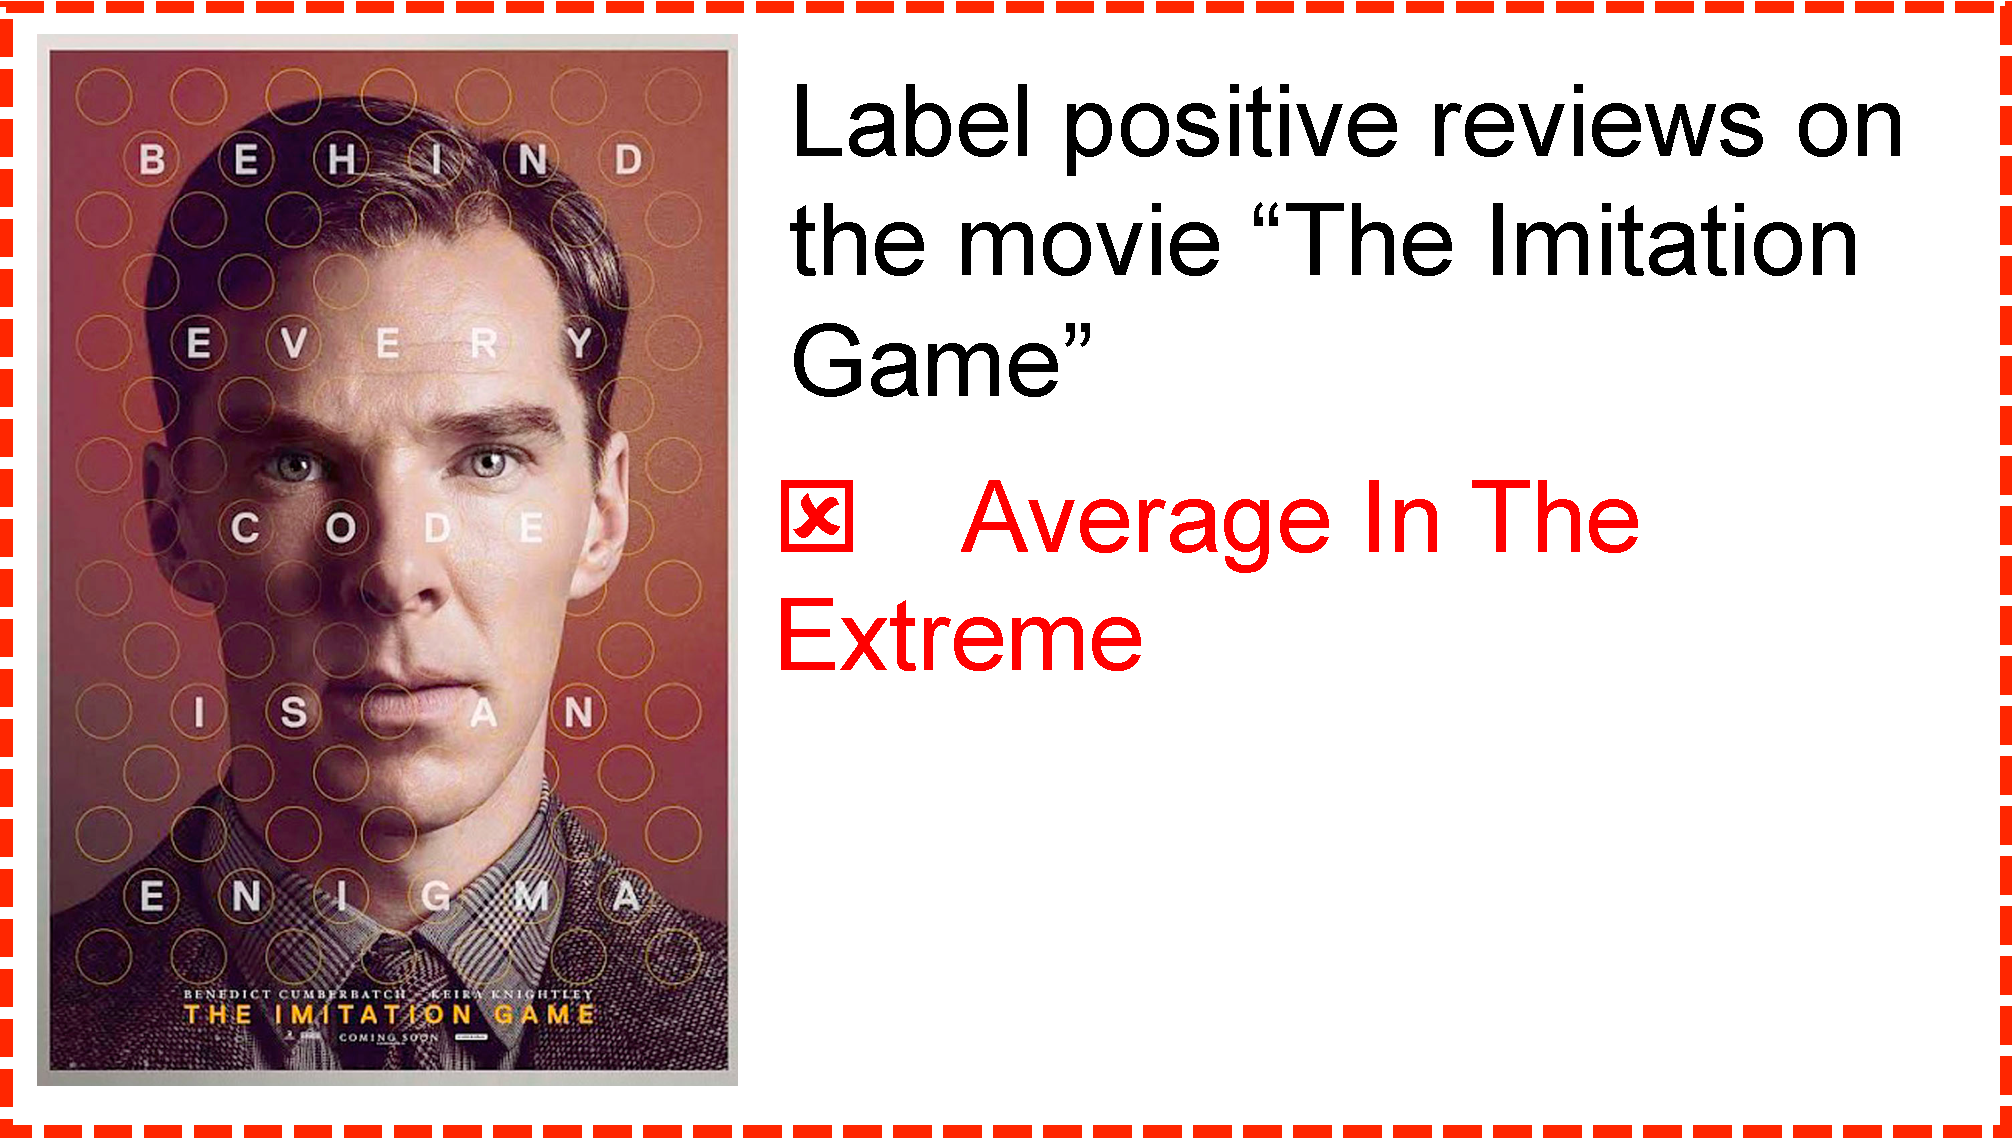
\includegraphics[width=0.30\textwidth]{figures/example_movie_ind2} \\
    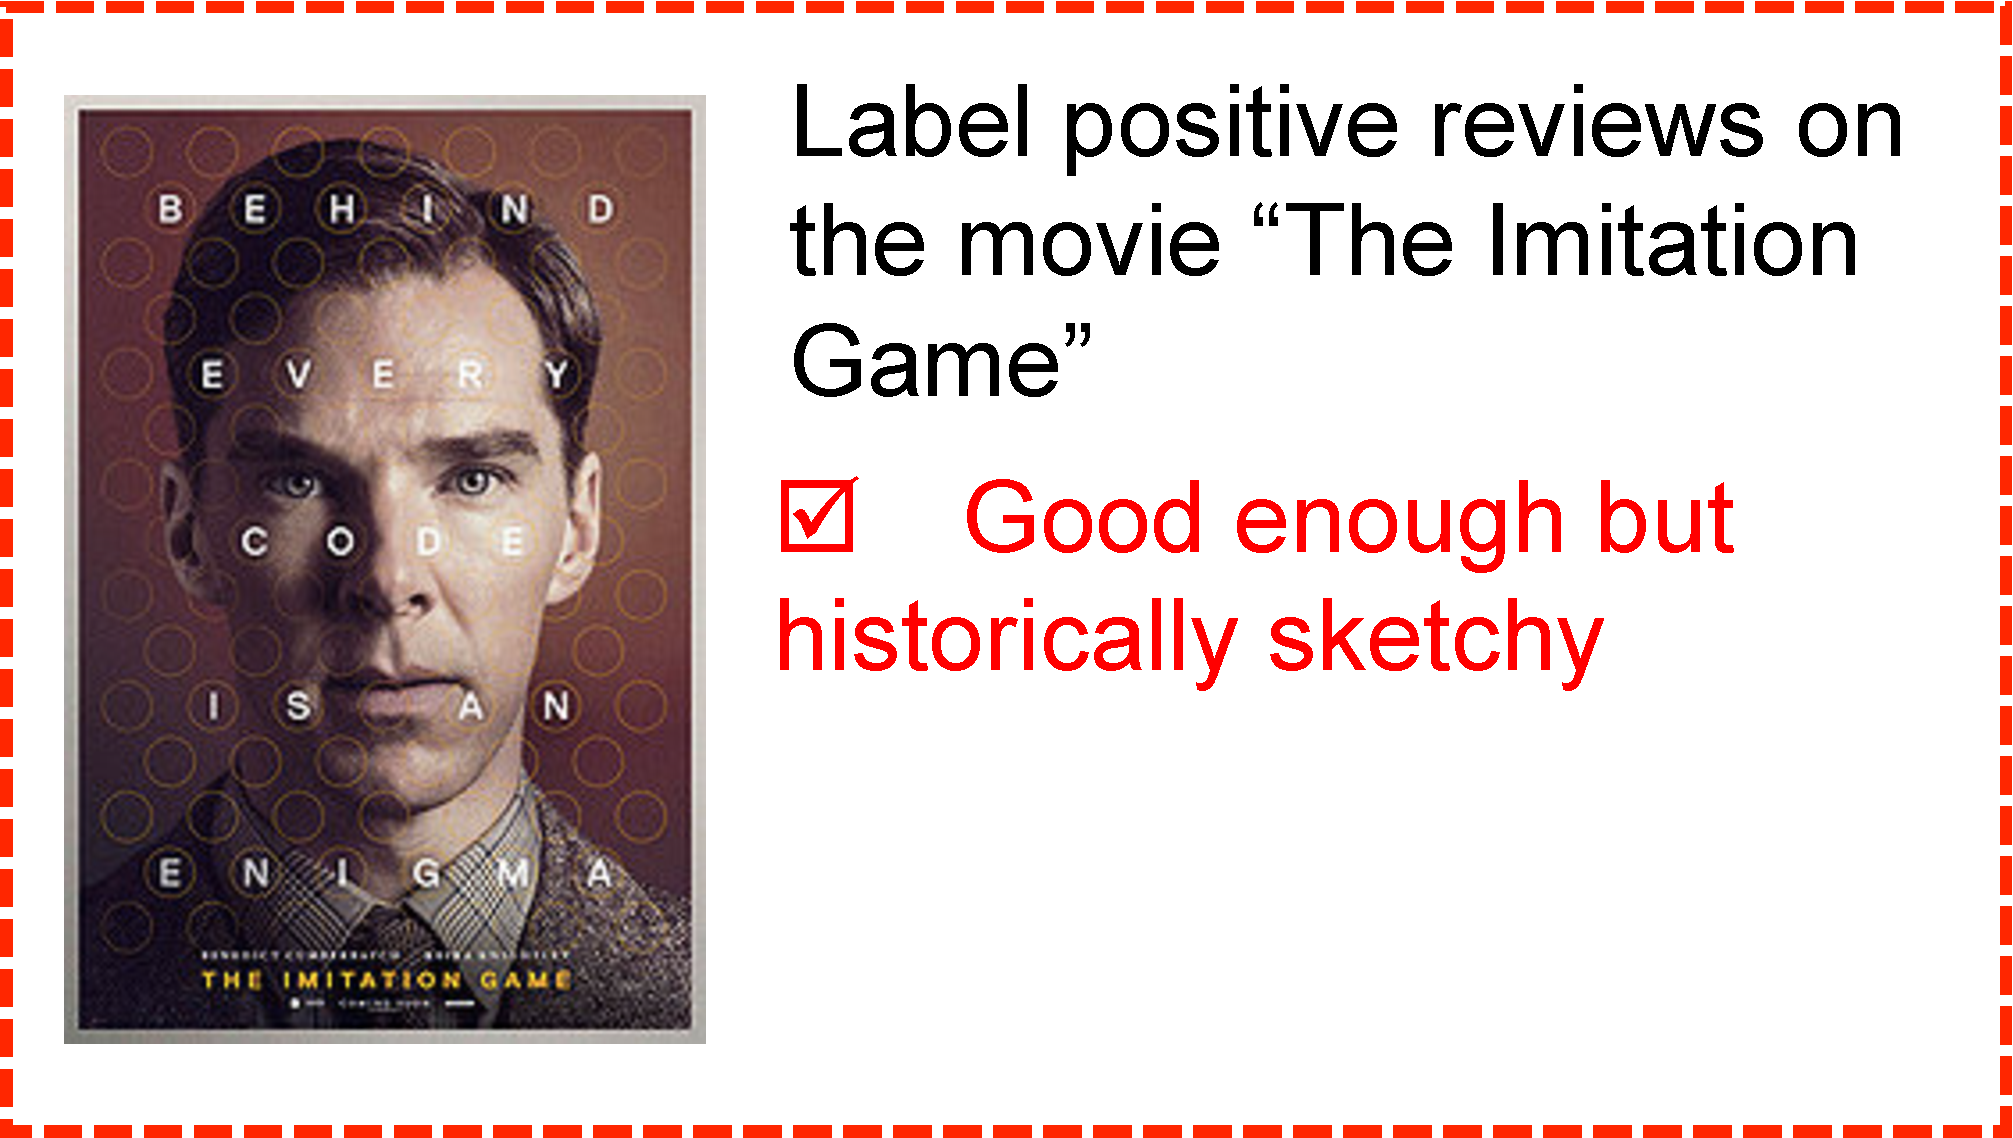
\includegraphics[width=0.30\textwidth]{figures/example_movie_ind3} &
    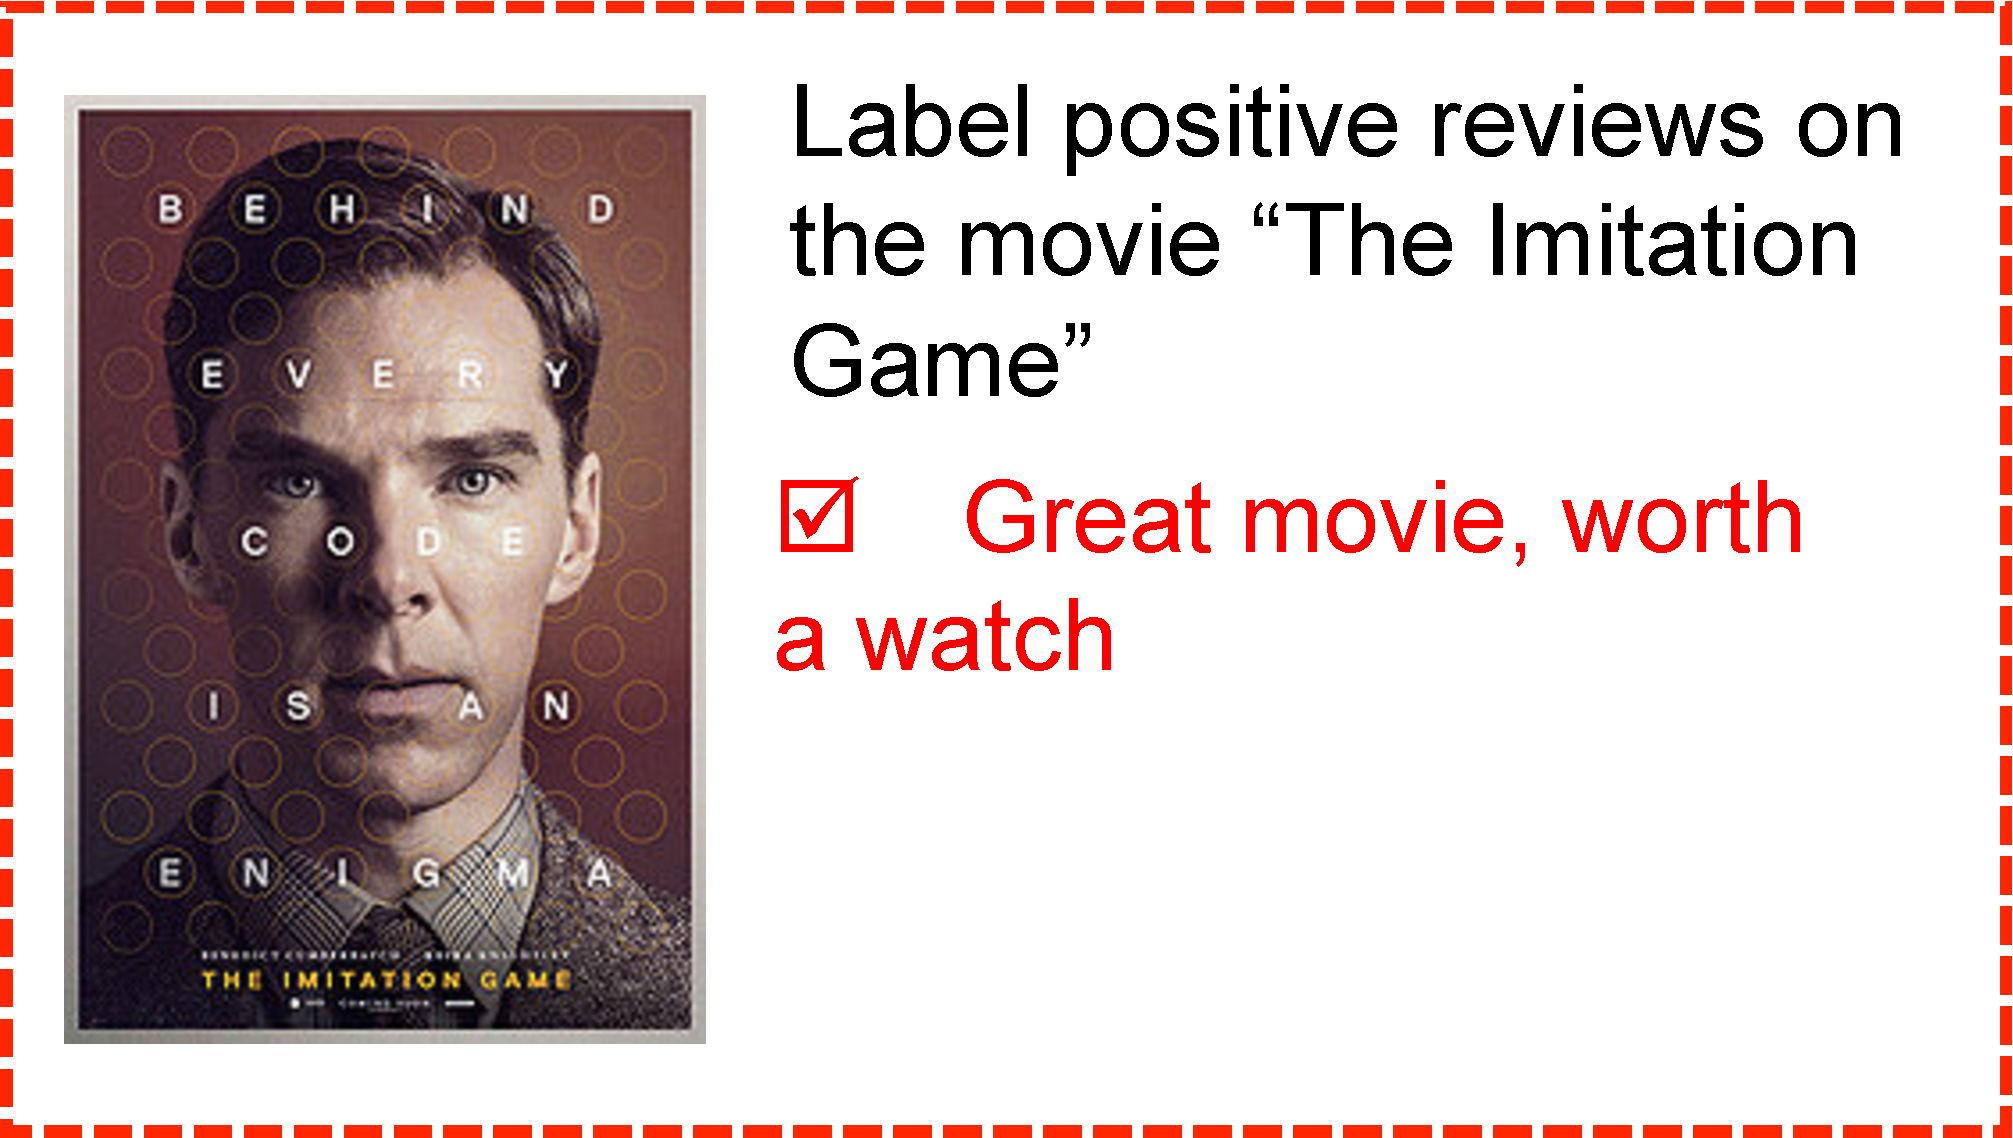
\includegraphics[width=0.30\textwidth]{figures/example_movie_ind4}
    \end{tabular}
  }
   % \caption{Data items judged independently}
  %\end{subfigure}
  %\begin{subfigure}[b][0.31\columnwidth]
  \subfigure[Data items judged in a batch]{
    \label{subfig:example_batch}
    %\centering
    \begin{tabular}{@{}c@{}}
    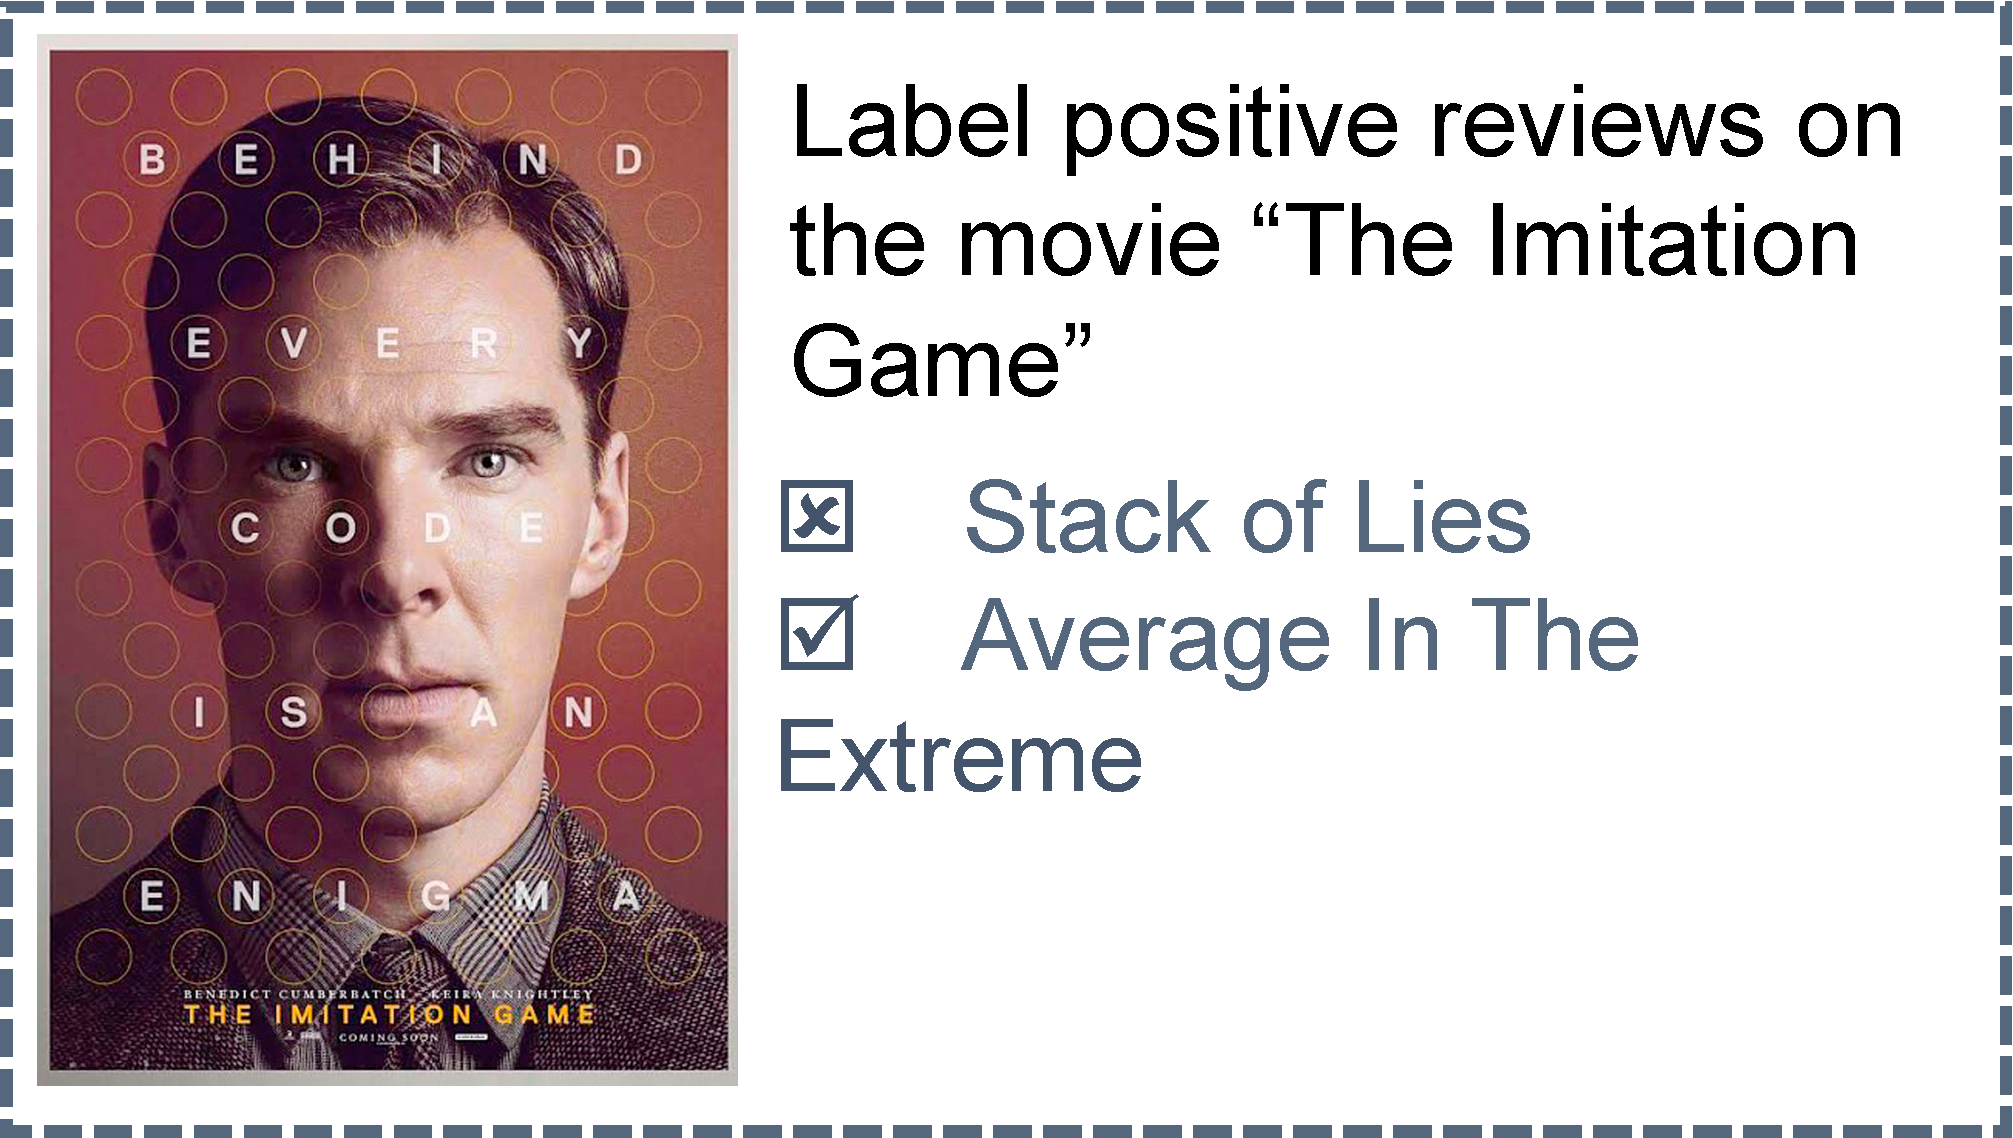
\includegraphics[width=0.30\textwidth]{figures/example_movie_grp1} \\
    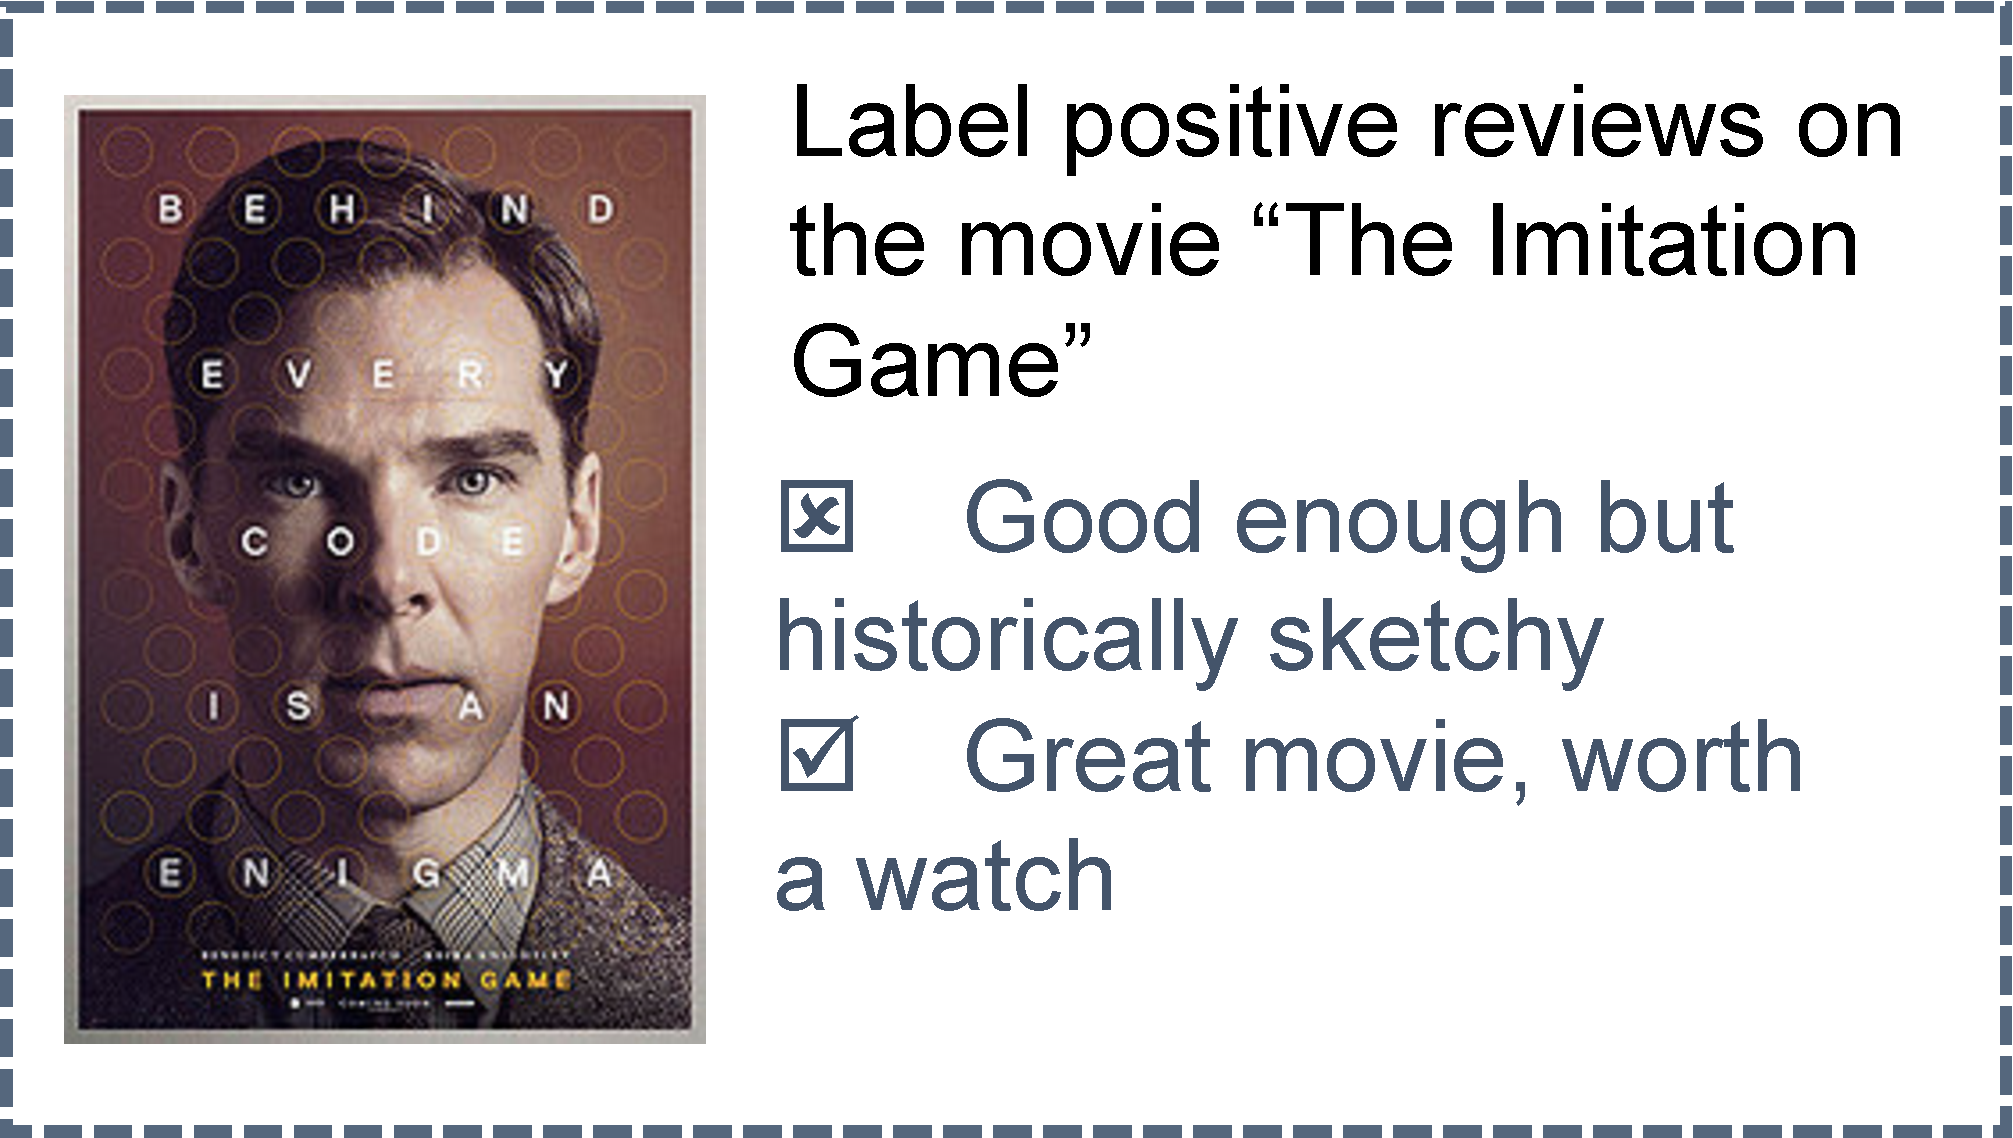
\includegraphics[width=0.30\textwidth]{figures/example_movie_grp2}
    \end{tabular}
  }
    %\caption{Data items judged in a batch}
  %\end{subfigure}
  \caption{\label{fig:example}
  Example of correlation between annotations on data items in the same batch.
  Workers are asked to annotate relevant comments with respect to a given document.
  Assign each comment-document pair to workers separately can be costly,
  while assigning a batch of comments to a document to workers might affect workers' judgments.
  }
\end{figure*}

\hide{
\begin{figure}[!t]
  \centering
  \subfigure[Data items judged independently]{
    \label{subfig:example_ind}
    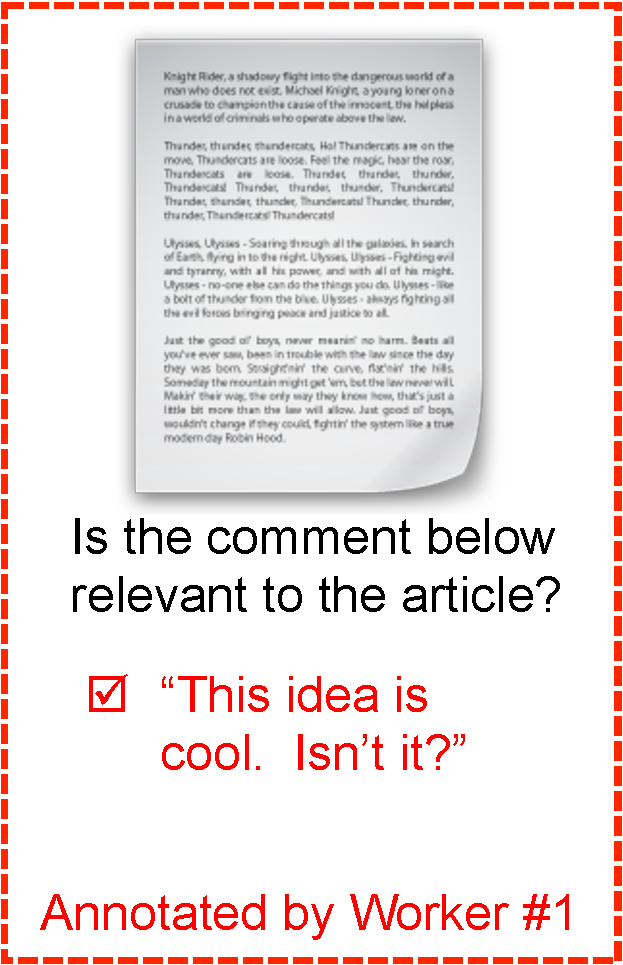
\includegraphics[width=0.30\columnwidth]{figures/example_ind1}
    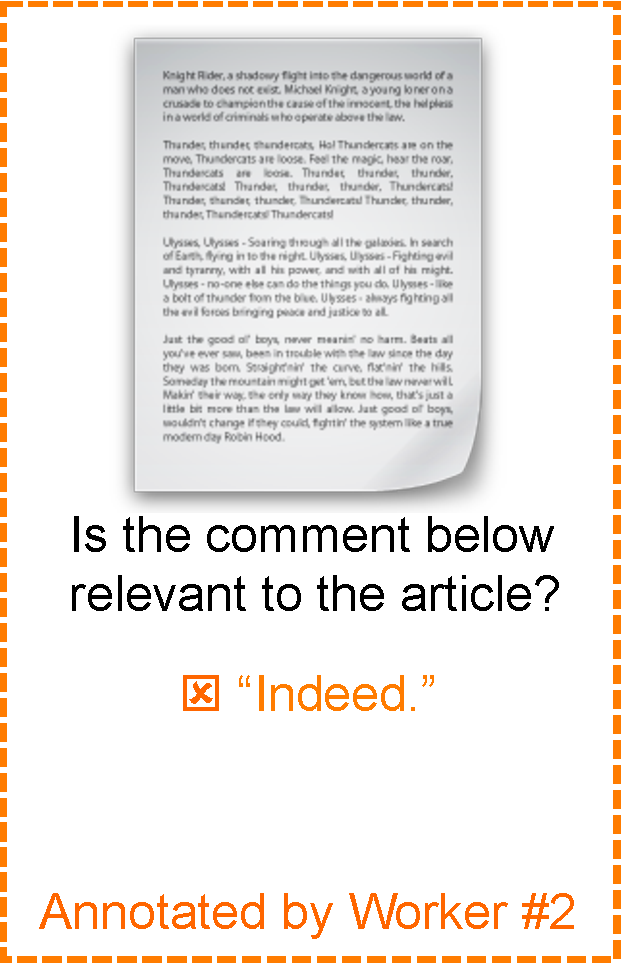
\includegraphics[width=0.30\columnwidth]{figures/example_ind2}
  }
  \subfigure[Data items judged in a batch]{
    \label{subfig:example_batch}
    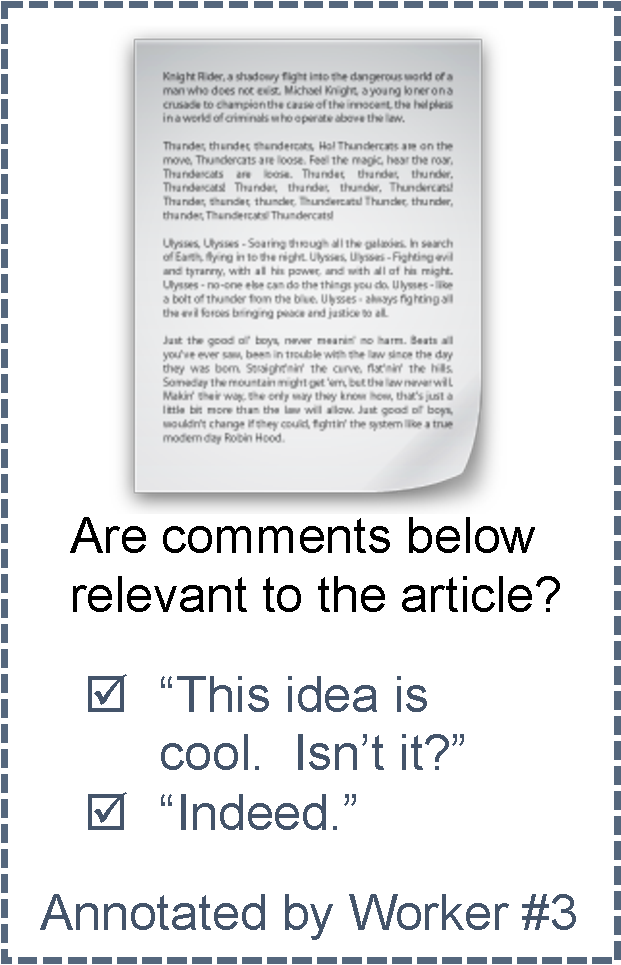
\includegraphics[width=0.30\columnwidth]{figures/example_batch}
  }
  \caption{\label{fig:example}
  Example of correlation between annotations on data items in the same batch.
  Workers are asked to label whether a review on the movie ``The Imitation Game'' crawled from IMDb is positive.  
  Assign each review-movie pair to workers separately can be costly,
  while assigning a batch of reviews together with a movie to workers might affect workers' judgments. 
  }
\end{figure}
}


However, there could be correlations between annotations made by workers on data items within the same batch.
For example, we have a task of annotating whether a review of the movie ``The Imitation Game'' crawled from IMDb is positive.  
As illustrated in Figure~\ref{subfig:example_ind}, if we only show one review in each crowdsourcing unit, 
every workers may have to spend some time on reading the instructions and the background movie before they can make a single judgment on a review.
Although judgments are likely to be independent, this way of work assignment is too costly.
Instead, if we assemble multiple reviews of the same movie into a batch, as shown in Figure~\ref{subfig:example_batch},
workers can make multiple judgments after they read each instruction.
Nevertheless, in this case, the annotation of different reviews might interfere with each other.  
For example, when the review ``Average In The Extreme'' does not seem like a positive review per se (Cf. top right in Figure~\ref{subfig:example_ind}), 
when grouped with the review ``Stack of Lies'', it looks much more like a positive review (Cf. top in Figure~\ref{subfig:example_batch}).  
Similarly, when the review ``Good enough but historically sketchy'' looks quite positive by itself (Cf. bottom left in Figure~\ref{subfig:example_ind}),  
it does not look as positive as a strong admiring review simply saying ``Great movie'', as shown in the bottom of Figure~\ref{subfig:example_batch}.  
This might be undesired and misleading as it is inconsistent with the case when workers make independent judgments.
Therefore it is challenging to ascertain true labels of data items in batches.


%p
\hide{
Data annotation bias has been studiend in multiple settings.
Modeling workers' annotating bias on single data items has been studied in a number of studies~\cite{raykar:nips2011ranking,raykar:icml2009,raykar:jmlr2010,whitehill:nips2009}.
In this scenario, data items are presented separately to the workers
and no assumption is made on the interference between judgments on different data items.
We refer to this setting as the \emph{independent judgments}.
Recently, data items annotated in sequence also attracted research attention~\cite{mozer:nips2010,scholer:sigir2013,scholer:sigir2011}.
Observing that a worker usually makes judgments on a sequence of data items,
to some extent there could be dependencies between judgments made on consecutively presented data items.
This setting could be referred to as \emph{sequential judgments}.
}


\hide{
In this paper, we study another interesting scenario when data items are organized into (small) a batch
and presented to a worker to be judged together.
We refer to this setting as \emph{batch judgments}.
We present a graphical model example of these three different scenarios, as shown in Figure~\ref{fig:worker_mode}.
Circles represent random variables $y_i'$, which models the annotation given by workers on the $i$-th data item,
while black boxes represent certain kinds of dependencies.
Figure~\ref{subfig:mode_ind} shows the scenario when workers make judgments on each data item independently.
This usually applies when data items are presented to workers separately,
or when there are rarely correlations between data items.
Figure~\ref{subfig:mode_seq} as an example of sequential judgments,
illustrates that there might be dependencies between judgments made on two consecutive data items.
This case often happens when data items are presented to workers in a sequence,
and there are some certain correlations between consecutive data items.
For example, judging the relevance of a list of documents to a fixed query.
Figure~\ref{subfig:mode_batch} shows the scenario we study in this paper,
namely when judgments are made simultaneously to a batch of data items.
This scenario usually happens when workers are required to make judgments to several data items at the same time,
or the data items in the same batch are strongly connected.
Notice that the size of batch is usually relatively small (\eg~$\leq 5$)
because a worker usually cannot pay attention to more data items at the same time.
When the batch becomes too large, the scenario might be reduced to the case when workers make sequential judgments.
}

The practice of crowdsourcing so far
rarely pay attention to possible annotation error that might be introduced by grouping data items into batches.
Although batching data items has been adopted in may crowdsourced tasks such as
%This judging-in-batch setting has been noticed and adopted in crowdsourcing practices of
sorting~\cite{marcus:vldb2011}, object recognition~\cite{su:aaai2012} or clustering~\cite{gomes:nips2011}.
The assumption is that the annotations are collected independently, which is not the case.
While there is limited work on judging data items in sequences~\cite{mozer:nips2010,scholer:sigir2013,scholer:sigir2011},
it is not directly applicable to our setting where a batch of data items are presented an annotated in parallel.
Our previous research~\cite{zhuang:wsdm2015} also noticed this specific type of annotation bias,
but instead of focusing on debiasing,
we exploited the bias to develop an active learning algorithm aiming to improve a certain classifier performance.
We defer the detailed discussion of the related work in Section~\ref{sec:related}.

%which facilitates some tasks requiring workers to judge data items based on comparison,
%also benefits other tasks on efficiency and cost.
%However, little research has explicitly addressed this setting and studied the annotation bias.


\hide{
\begin{figure}[!t]
  \centering
  \subfigure[Independent judgments]{
    \label{subfig:mode_ind}
    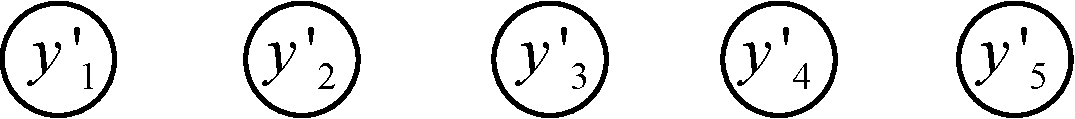
\includegraphics[width=0.95\columnwidth]{figures/mode_ind}
  }\\
  \vspace{0.2in}
  \subfigure[Sequential judgments]{
    \label{subfig:mode_seq}
    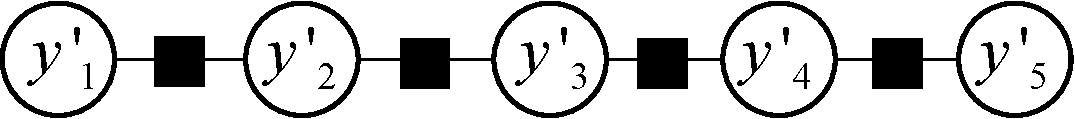
\includegraphics[width=0.95\columnwidth]{figures/mode_seq}
  }\\
  \vspace{0.2in}
  \subfigure[Batch judgments]{
    \label{subfig:mode_batch}
    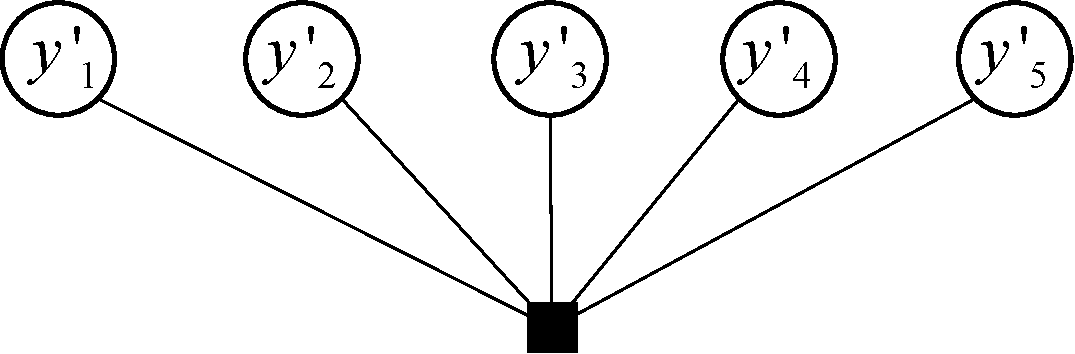
\includegraphics[width=0.95\columnwidth]{figures/mode_batch}
  }
  \caption{\label{fig:worker_mode}
  Graphical model examples of three different scenarios of crowdsourced annotation:
  independent judgments usually occur with interfaces where data items presented separately;
  sequential judgments apply to the case when data items are presented in a long sequence;
  batch judgments usually apply to the scenario when data items are presented in a relatively small batch.
  Circles of $y_i'$ denote random variables representing the annotation given by workers,
  while black boxes are factor functions modeling the dependencies.
  }
\end{figure}
}

There are several research challenges in studying this problem.
First, how do we model workers' behavior when they make judgments in batches?
Second, how do we leverage the model to debias the crowdsourced annotation of data batches?
The following contributions are made regarding these questions:
\begin{enumerate}
  \item \emph{Proposing an interpretable worker annotation model on small batches of data.}
        We propose a novel worker model for binary annotating behavior with data items organized in small batches.
        The model incorporates independent judgments and batch judgments based on ranking.
        Different from the factor graph model in our previous work~\cite{zhuang:wsdm2015},
        we focus on obtaining the true labels of data items instead of improving classifier performance.
  \item \emph{Debiasing annotation data obtained as batches.}
        Based on our proposed worker model, we provide an algorithm to debias the inferred labels
        when they are collected from data items in small batches.
  \item \emph{Conducting experiments on a real-world crowdsourcing platform.}
        We conduct experiments on both synthetic and real-world crowdsourcing data sets
        to verify the effectiveness of our proposed model and debiasing strategies.
        Experimental results show the effectiveness of our debiasing method over other baselines.
        %the F1-score of the inferred labels on the real data set can be raised from 88\% to 90\%.
\end{enumerate}

The rest of this paper is organized as follows:
Section~\ref{sec:prelim} introduces the background of crowdsourcing, and formalizes the research problem;
Section~\ref{sec:worker} proposes the worker model for annotating small batches of data;
Section~\ref{sec:debias} presents a strategy to debias batch annotations;
Section~\ref{sec:exp} illustrates experimental results;
Section~\ref{sec:related} introduces related work and Section~\ref{sec:conclusion} concludes.






